\subsection{Reaktyvus programavimas bei įvykių kaupimas kartu}

Šiame poskyryje bus siekiama pasiekti darbo tikslą - pritaikyti reaktyvaus programavimo principus įvykių kaupimo sistemose taip, jog skaitymo modelis būtų kuriamas tik komponavimo būdu, neturėtų būsenos, tai yra visos operacijos su duomenų baze būtų paslėptos. Pirmiausia bus aprašyta problema, su kuria susiduriama kuriant įvykių kaupimo sistemos skaitymo modelį naudojantis ``RailsEventStore'' biblioteka. Vėliau bus pristatyti kuriamos patobulintos bibliotekos reaktyvūs operatoriai bei jų panaudojimo atvejai, aprašyta kūrimo eigos metodika, iššūkiai bei jų sprendimai, suformuluoti apribojimai.

\subsubsection{Įprasto būdo kurti įvykių kaupimo sistemas problema}

Praeitame poskyryje buvo pademonstruotas įvykių kaupimo sistemos skaitymo modelio kūrimas panaudojant egzistuojančią biblioteką. Tačiau toks bibliotekos panaudojimas nėra deklaratyvus, programuotojui tenka rašyti darbo su duomenų baze operacijas. Norima tokį pašalinį efektą paslėpti, jog būtų galima koncentruotis tik ties sprendžiama problema.

Remiantis G. Salvaneschi empiriniu tyrimu apie programos, paremtos reaktyviu programavimu, suprantamumą \cite{Salvaneschi:2014:ESP:2635868.2635895}, tai galėtų sumažinti programuotojo daromų klaidų skaičių bei pagerinti programos suprantamumą.

\subsubsection{Pasiruošimas kurti biblioteką}

Norint išspręsti minėtą problemą ir sukurti patogią naudotis biblioteką, pirmiausia reikia atsakyti į šiuos klausimus:

\begin{itemize}
  \item Kaip įvykiai bus saugojami ir publikuojami?
  \item Kaip atrodys skaitymo modelio kvietimas?
  \item Kaip atrodys skaitymo modelio kūrimo aprašas?
  \item Kokie reaktyvūs operatoriai bus realizuoti?
  \item Kurie reaktyvūs operatoriai turi paslėpti operacijas su duomenų saugykla?
\end{itemize}

Sekančiuose skyriuose atsakysime į šiuos klausimus.

\subsubsection{Įvykių saugojimas ir publikavimas}

Įvykių saugojimui pasirenkamas aktyvaus įrašo projektavimo šablonas, kuris buvo nagrinėtas literatūros analizėje. Įvykių publikavimui galima panaudoti ``rails\_event\_store\_active\_record''\footnote{https://github.com/arkency/rails\_event\_store\_active\_record} biblioteką. Ją pagal nutylėjimą naudoja ``RailsEventStore'' biblioteka.

Tarkime turime domeno sritį bankininkystė ir vartotojas gali atlikti šias operacijas, kurias atvaizduotų atitinkami įvykiai sistemoje:

\begin{itemize}
  \item \lstinline|AccountCreated| - susikurti sąskaitą, kuri turėtų unikalų sąskaitos identifikatorių ir einamąjį balansą.
  \item \lstinline|MoneyDeposited| - įnešti pinigus į sąskaitą.
  \item \lstinline|MoneyWithdrawn| - išsiimti pinigus.
\end{itemize}

Įvykio publikavimo pavyzdys:

\begin{lstlisting}
stream_name = "account"
event = AccountCreated.new(data: {
          account_id: ``LT121000011101001000''
        })
EventStore::EventRepository.new.create(event, stream_name)
\end{lstlisting}

\subsubsection{Skaitymo modelio kvietimas}

Patogiam užklausų rašymui, pasirenkamas aktyvaus įrašo projektavimo šablonas, kuris buvo nagrinėtas literatūros analizėje.

Norint surasti sąskaitą \lstinline|Account| pagal unikalų identifikatorių užtenka iškviesti:

\begin{lstlisting}
  Account.find_by(account_id: 'LT121000011101001000')
\end{lstlisting}

Norint atvaizduoti sąskaitas, kurios buvo atidarytos paskutinį mėnesį ir išrūšiuoti pagal naujumą užtenka iškviesti:

\begin{lstlisting}
  Account.filter(created_at: 1.month.ago..Time.current).order(created_at: :desc)
\end{lstlisting}

\subsubsection{Skaitymo modelio kūrimo aprašas}

Tarkime, jog norime sukurti skaitymo modelį, kuris atvaizduotų dabartinį vartotojo sąskaitos balansą. Skaitymo modelio kūrimo kodas turėtų atrodyti taip:

\begin{lstlisting}
account_view =
  Stream.new(AccountCreated, MoneyDeposited, MoneyWithdrawn).
    as_persistent_type(Account).
    init( -> (state) { state.balance = 0} ).
    when(MoneyDeposited), -> (state, event) { state.balance += event[:data][:amount] }).
    when(MoneyWithdrawn), -> (state, event) { state.balance -= event[:data][:amount] })
\end{lstlisting}

Verta pažymėti, jog čia nėra nė vienos operacijos su duomenų saugykla. Jeigu būtų sukurta vartotojo sąskaita su kodu ``LT121000011101001000'', dabartinį sąskaitos balansą galėtume gauti tiesiog iškvietę \lstinline|Account.find_by(account_id: 'LT121000011101001000').balance|

\subsubsection{Reaktyvūs operatoriai}

Kuriant biblioteką pasirinkta įgyvendinti šiuos operatorius:

\begin{itemize}
  \item \lstinline|merge(another_stream)| - srautų sujungimo operatorius. Šis operatorius sujungia 2 srautus į vieną.
  \item \lstinline|filter(predicate_function)| - filtravimo operatorius. Operatorius tikisi funkcijos, kuri pritaiko įvykį šiai funkcijai ir tikisi \lstinline|boolean| tipo atsakymo.
  \item \lstinline|map(transform_function)| - transformavimo operatorius. Operatorius tikisi funkcijos, kuri transformuoja įvykį.
  \item \lstinline|init(initial_state_function)| - pradinės reikšmės operatorius. Operatorius išsaugo pradinę skaitymo modelio būseną duomenų saugykloje, jei ji dar nesukurta.
  \item \lstinline|when(event_type, state_change_function)| - tipo atitikimo operatorius. Nutikus tam tikram tipo \lstinline|event_type| įvykiui, duomenų saugykloje išsaugoma tarpinė skaitymo modelio būsena pritaikant būsenos pakeitimo funkciją.
  \item \lstinline|each(state_change_function)| - iteratoriaus operatorius. Funkcionalumas identiškas tipo atitikimo operatoriui \lstinline|when|, tačiau būsenos keitimo funkcija pritaikoma bet kokiam įvykiui.
\end{itemize}

Šie operatoriai bus plačiau paaiškinti ir pademonstruoti aprašant realizacijos detales.

\subsubsection{Pagrindiniai realizacijos iššūkiai}

Apsibrėžus kuriamos bibliotekos norimą pasiekti funkcionalumą bei naudojimosi sintaksę, kyla daugiau klausimų:

\begin{itemize}
  \item Kaip stebėti įvykius sistemoje?
  \item Kaip realizuoti srautą bei reaktyvius operatorius?
  \item Kaip išsaugoti tarpinę skaitymo modelio būseną paslepiant operacijų su duomenų saugykla detales?
\end{itemize}

Sekančiame skyriuje aptarsime bibliotekos realizacijos detales bei kertinius sprendimus, atsakančius į išsikeltus klausimus.

\subsubsection{Realizacijos detalės}

Analizuojant reaktyvaus programavimo bibliotekas, buvo pastebėta, jog jos naudoja stebėtojo projektavimo šabloną. Remiantis analizės rezultatais apsibrėšime klases, kurių reikia funkcionalumui realizuoti. Kuriamos bibliotekos klasių priklausomybių diagrama pavaizduota \ref{img:class_diagram} paveikslėlyje.

\begin{figure}[H]
    \centering
    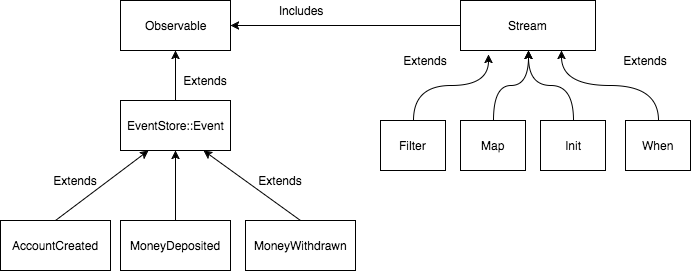
\includegraphics[scale=0.6]{img/class_diagram}
    \caption{Kuriamos bibliotekos klasių priklausomybių diagrama}
    \label{img:class_diagram}
\end{figure}

\textbf{Įvykių stebėsenos realizacija}

\lstinline|EventStore::Event| išplečia \lstinline|Observable| modulį ir šiuo atveju yra tema. Kiekvienas įvykio tipas sistemoje yra kuriamas paveldint \lstinline|EventStore::Event| klasę:

\begin{lstlisting}
class AccountCreated < EventStore::Event
end

# arba

AccountCreated = Class.new(EventStore::Event)
\end{lstlisting}

Kadangi tema yra klasė, o ne objektas (tokiu atveju programuotojui pačiam tektų informuoti stebėtojus), verta atskirai panagrinėti \lstinline|EventStore::Event| klasės objekto metodą \lstinline|emit|:

\begin{lstlisting}
def emit
  self.class.changed
  self.class.notify_observers(self.to_h)
end
\end{lstlisting}

Išplečiant klasę \lstinline|Observable| moduliu, pastarosios metodai yra pridedami klasei, o ne tos klasės objektui. Čia galima panaudoti introspekciją ir sužinoti kokio tipo objektui metodas yra kviečiamas. Taip informuojami visi stebėtojai, kurie prenumeruoja šią temą. Šis metodas yra iškviečiamas iškart po to kai įvykis būna įrašytas į duomenų saugyklą naudojantis anksčiau minėtu įvykių publikavimo mechanizmu. Galime pažvelgti į klasės \lstinline|EventRepository|, atsakingos už įvykių publikavimą, metodą \lstinline|create|:

\begin{lstlisting}
def create(event, stream_name)
  data = event.to_h.merge!(stream: stream_name)
  adapter.create(data)

  # Notify observers of new event
  event.emit if event.respond_to?(:emit)

  event
end
\end{lstlisting}

Kai tik įvykis išsaugomas duomenų saugykloje, visi įvykio prenumeratoriai yra informuojami apie naują įvykį sistemoje.

\textbf{Skaitymo modelio kūrimo aprašo realizacija}

Skaitymo modelis yra kuriamas pasinaudojant duomenų srautais. Inicializuojant duomenų srautą \lstinline|Stream.new(*sources)|, konstruktoriuje apibrėžiami prenumeruojami įvykiai:

\begin{lstlisting}
sources.each { source.add_observer(self) }
\end{lstlisting}

Srautas geba pats pasirūpinti, jog būtų informuotas apie naujus įvykius sistemoje.

Srautas taip pat realizuoja svarbų metodą \lstinline|update|, kuris yra visada iškviečiamas gavus naują įvykį.

Kiekvienas reaktyvus operatorius yra kuriamas labai panašiai, todėl pateiksime tik porą operatorių realizaciją:

\begin{lstlisting}
def filter(blk)
  Filter.new(self, blk)
end

def when(event_type, blk)
  When.new(self, event_type, blk)
end
#...
\end{lstlisting}

Grąžinama nauja atitinkama klasė, kuri paveldi \lstinline|Stream| srautą. Verta pastebėti, jog perduodamas ir pradinis srautas. Taigi srautas \lstinline|Stream| tuo pačiu metu gali būti ir stebėtojas, ir tema.

\textbf{Kuriamo skaitymo modelio tipo operatorius}

Norint išsaugoti tarpinę skaitymo modelio būseną duomenų saugykloje, reikia žinoti skaitymo modelio tipą bei jo unikalų identifikatorių.

\lstinline|as_persistent_type(resource_type, unique_resource_identifier)| yra srauto metodas, kuris įsimena kuriamo skaitymo modelio tipą bei jo unikalų identifikatorių. Naudojant reaktyvius operatorius, modelio tipas ir unikalus identifikatorius yra automatiškai perduodamas naujam reaktyvaus operatorio srautui. Bendruoju atveju, unikalus identifikatorius gali būti nuspėtas. Tarkime, jeigu kuriamas vartotojo sąskaitos skaitymo modelis \lstinline|Account|, unikalus identifikatorius greičiausiai bus \lstinline|account_id|. Kartais gali atsirasti noras kurti sudėtingesnius skaitymo modelio vaizdus. Tarkime, programos vartotojas gali turėti kelias sąskaitas. Tokius atveju unikalus identifikatorius turėtų būti pora \lstinline|user_id, account_id| - vartotojo kodas ir sąskaitos kodas. Norint sukurti tokį skaitymo modelį, užtektų kuriamo skaitymo modelio aprašo srautui iškviesti \lstinline|as_persistent_type(Account, [:account_id, :user_id])|. Tvarka šiuo atveju nesvarbi. Metodas grąžina pasinaudoja metodų apjungimo principu, tai yra grąžina objektą, kuriam buvo iškviestas.

Įprastai programuotojas turi apsirašyti aktyvaus įrašo modelį pats \lstinline|class Account < ActiveRecord::Base; end|. Tačiau čia gali pasitarnauti meta programavimas \cite{Olsen:2007:DPR:1349728}, kuris leidžia programuotojams būti produktyvesniems generuojant dalį kodo. Šiuo atveju biblioteka leidžia paduoti ne tik jau aprašytą aktyvaus įrašo tipą, bet priima tiek eilutės, tiek simbolio tipą ir gali dinamiškai paveldėti aktyvaus įrašo bazinį tipą panaudojant refleksija:

\begin{lstlisting}
@resource_type =
  if defined_stream_type.is_a? String
    Object.const_set(dynamic_name, Class.new(ActiveRecord::Base))
  elsif defined_stream_type.is_a? Symbol
    Object.const_set(defined_stream_type.to_s.capitalize, Class.new(ActiveRecord::Base))
  else
    defined_stream_type
  end
\end{lstlisting}

\textbf{Filtravimo operatorius}

Filtravimo operatorius \lstinline|filter| priima predikatą, tai yra tam tikrą sąlygą. Jeigu ši sąlyga yra teisinga, įvykis yra perduodamas toliau visiem jo prenumeratoriams. Šis funkcionalumas realizuojamas pasinaudojant objektinio programavimo sąvybe polimorfizmu. Tėvinės klasės metodas \lstinline|update| yra perrašomas ir pakeitimai perduodami tik tada kai sąlyga yra išpildyta:

\begin{lstlisting}
class Filter < Stream
  def initialize(source, blk)
    @resource_type = source.resource_type
    @unique_resource_identifier = source.unique_resource_identifier
    @block = blk
    source.add_observer(self)
  end

  def update(event)
    occur(event) if @block.call(event)
  end
end
\end{lstlisting}

Galime panagrinėti šio reaktyvaus operatoriaus panaudojimo atvejį. Tarkime vartotojas sistemoje gali tiek nusipirkti prekę, tiek užsisakyti, jog prekė būtų pagaminta pagal užsakymą. Gali kilti noras konstruoti skaitymo modelį, apjungiantį juos abu bei turint papildomų sąlygų. Pavyzdžiui vartotojui gali būti suteikiami kreditai už sėkmingą pirkimą tik tada, kai:

\begin{itemize}
  \item Pirkinio vertė yra didesnė nei 100 eurų.
  \item Specialaus užsakymo vertė yra daugiau nei 50 eurų.
\end{itemize}

Tokį duomenų srautą galima konstruoti panaudojant reaktyvų filtravimo operatorių \lstinline|filter| kaip:

\begin{lstlisting}
  product_orders_eligible_for_bonus =
    Stream.new(ProductPurchased).
                filter( -> (event) event[:data][:price_paid] > 100)

  job_orders_eligible_for_bonus =
    Stream.new(JobOrderPurchased).
               .filter( -> (event) event[:data][:price_paid] > 50)
\end{lstlisting}

\textbf{Srautų sujungimo operatorius}

Apibrėžiant filtravimo operatorių, buvo sukurti 2 srautai, kurie yra filtruojami skirtingi. Norėdami pritaikyti bendrus veiksmus jiems, turime turėti galimybę juos sujungti. Šių filtruotų srautų sujungimo operatorius \lstinline|merge| atrodytų kaip:

\begin{lstlisting}
  merged_stream = product_orders_eligible_for_bonus.merge(job_orders_eligible_for_bonus)
\end{lstlisting}

Metodo \lstinline|merge| realizacija yra naujo srauto sukūrimas, panaudojant 2 srautus:

\begin{lstlisting}
def merge(another_stream)
  Stream.new(self, another_stream)
end
\end{lstlisting}

\textbf{Pradinės reikšmės operatorius}

\lstinline|init| metodas veikia kaip inicializatorius. Jeigu skaitymo modelis dar nėra saugomas duomenų saugykloje, sukuriant įrašą bus nustatoma pradinės įrašo reikšmės. Šiuo atveju sąskaitos balansas bus 0. Metodas priima \lstinline|lambda| funkciją, kuri bus iškviesta inicializavimo metu.

\begin{lstlisting}
def update(event)
  check_resource_type_presence

  entity_id_hash = extract_entity_id(event)

  if !@resource_type.where(entity_id_hash).exists?
    resource = @resource_type.new(event[:data])
    @block.call(resource)
    resource.save!
  end

  occur(event)
end
\end{lstlisting}

Čia \lstinline|update| metodas yra iškviečiamas kiekvieną kartą, kai duomenų srautas gauna naują įvykį, o stebėtojas jį prenumeruoja. \lstinline|Init| tipo srautas saugo informaciją apie kuriamą skaitymo modelio tipą, todėl iš gauto įvykio gali išgauti unikalaus identifikatoriaus informaciją. Jeigu toks skaitymo modelis dar nėra sukurtas sistemoje, naujas įrašas yra sukonstruojamas, pritaikoma būsenos keitimo funkcija ir programos tarpinė būsena yra išsaugoma duomenų saugykloje. Įvykis visada perduodamas toliau visiems prenumeratoriams.

\textbf{Tipo atitikimo operatorius}

Operatorių \lstinline|when(event_type, blk)| galima vadinti tipo atitikimo operatoriumi. Perduodamas \lstinline|lambda| blokas bus iškviestas tik tada kai sistemoje įvykusio įvykio tipas bus toks, koks yra apibrėžtas.

Jeigu tipai atitinka ir skaitymo modelio tarpinė būsena dar nėra saugoma duomenų saugykloje, šio operatoriaus realizacija yra identiška \lstinline|init| operatoriaus realizacijai.

Jeigu tipai atitinka ir skaitymo modelio tarpinė būsena jau yra saugoma duomenų saugykloje, būsena užklausiama, modifikuojama panaudojus būsenos keitimo funkciją, o gautas tarpinis rezultatas išsaugomas duomenų saugykloje:

\begin{lstlisting}
resource = @resource_type.where(entity_id_hash).first
@block.call(resource)
resource.save!
\end{lstlisting}

\textbf{Iteratoriaus operatorius}

Kartais gali vertėti klausytis kelių įvykių šaltinių ir jiems pritaikyti bendras operacijas. Tarkime norime atnaujinti informaciją paieškos duomenų saugykloje, kai pasikeičia kokia nors svarbi informacija apie produktą. Tokį funkcionalumą, galėtume išreikšti kaip:

\begin{lstlisting}[]
  Stream.new(ProductImageUploaded, ProductInformationChanged)
      .as_persistent_type(Product)
      .each( -> (state, event) state.reindex )
\end{lstlisting}

Iteratoriaus operatoriaus \lstinline|each| realizacija yra identiška tipo atitikimo operatoriui. Vienintelis skirtumas, jog būsenos keitimo funkcija yra pritaikoma visems prenumeruojamiems įvykiams.

\textbf{Skirtingi būdai struktūrizuoti skaitymo modelio aprašą}

Iš esmės \lstinline|lambda| blokas yra vykdomas, kai jam iškviečiamas \lstinline|call| metodas. Kadangi aprašyti operatoriai priima \lstinline|lambda| bloką kaip parametrą, esti papildomi būdai perduoti juos.

Galima apsirašyti kintamąjį:

\begin{lstlisting}
  variable = -> (event) { }
\end{lstlisting}

Taip pat galima apsirašyti klasę, kuri turi \lstinline|call| metodą:

\begin{lstlisting}
  class Denormalizers::ReadModelType::Event
    def call(state, event)
      # implementation
    end
  end
\end{lstlisting}

Lankstumas suteikia galimybę laisvai struktūrizuoti kodą, sutrumpinti skaitymo modelio kūrimo aprašą, kas gali pagerinti projekto priežiūrą, skaitomumą bei programuotojo produktyvumą.

\subsubsection{Apribojimai}

Sujungus reaktyvaus programavimo ir įvykių kaupimo principus ir sukūrus biblioteką, pastebėti tam tikri apribojimai, kuriuos verta paminėti:

\begin{itemize}
  \item Saugant tarpinę skaitymo modelio tipo būseną reikalingas ne tik tipas, bet ir to skaitymo modelio unikalus identifikatorius. Šis identifikatorius paimamas iš prenumeruojamo įvykio nešamos informacijos. Dėl šio priežasties kiekvienas prenumeruojamas įvykis privalo turėti šią informaciją.
  \item Srautas nėra baigtinis, operatorių funkcijos pritaikomos tik nutikus įvykiui, todėl neįmanoma užklausti pagal kintantį laiką. Pavyzdžiui, negalėtume sukurti tam tikro skaitymo modelio, kuris vaizduotų paskutinių 24h operacijas. Norint tikslumo, tam derėtų pasinaudoti įvykių saugyklos adapteriu \lstinline|EventRepository|, skaityti paskutinius įvykius sistemoje ir kurti laikiną skaitymo modelį nesinaudojant biblioteka.
  \item Sukurta biblioteka niekada nesunaikina tarpinės skaitymo modelio būsenos. Esant reikalui identifikuoti sunaikintą būseną, galima prenumeruoti naikinimo įvykį ir turėti tam tikrą \lstinline|status| identifikatorių, kuris pažymėtų skaitymo modelio būseną sistemoje. Pavyzdžiui, elektroninėje parduotuvėje gali tekti žinoti ar produktas pradedamas kelti, įkeltas, suspenduotas ar ištrintas.
\end{itemize}

\subsubsection{Pavyzdinis projektas panaudojantis aprašytą biblioteką}

Pilnas išeities kodas yra prieinamas skaitmeninėje laikmenoje, kuri yra pridėta prie darbo. Projekto aplanko pavadinimas yra \lstinline|cappuccino|. Pagrindinės nuorodos:

\begin{itemize}
  \item \lstinline|README.md| - aprašytos diegimo instrukcijos, testų paleidimo instrukcijos bei bibliotekos naudojimosi instrukcijos.
  \item \lstinline|app/lib/event_store| - bibliotekos failai, reikalingi įvykių publikavimui.
  \item \lstinline|app/lib/cappuccino| - bibliotekos failai, reikalingi kuriant skaitymo modelį panaudojant reaktyvųjį programavimą.
  \item \lstinline|spec/lib| - testai, užtikrinantys korektišką bibliotekos elgesį, tai yra validuojantys funkcionalumą.
\end{itemize}
